\documentclass[11pt, a4paper, oneside]{memoir}
\usepackage{float}
\usepackage{graphicx}
\graphicspath{{img/}}

\include{config}
\include{acro}

\title{\Huge Reducción polinomial de 3DM a Partition}


\author{Airam Rafael Luque León \and
Juan Salvador Magariños Alba \and
Lucas Hernández Abreu \and
Alejandro García Perdomo
}


\begin{document}
\maketitle

\chapter{}

\section{Problemas involucrados}

\subsection*{3DM}

\noindent ENTRADA: 3 conjuntos de elementos $W$, $X$ y $Y$, con  $|W|$ = $|X|$ = $|Y|$ = $q$, y $M$, que es un conjunto de tripletas $(w,x,y)$ formadas por \(w \in W, x \in X,y \in Y\), con $\mid$M$\mid$ = $k$. 

\noindent PREGUNTA: ¿Existe un emparejamiento tridimensional M' $\subseteq$ M con $\mid$M'$\mid$ = $q$, en el que todos los elementos de $W$, $X$, $Y$ aparezcan una única vez? 
\subsection*{Partition}

\noindent ENTRADA: Un conjunto de números $A$, con \(a \in A\), tal que \(s(a)\in Z^{+}\).

\noindent PREGUNTA: ¿Existe un conjunto $A'$ que cumpla la siguiente condición? \[ \sum_{a\in A'}s(a)= \sum_{a\in A - A'}s(a)\] 


\section{Demostración de NP-completitud}

\vspace{0.5cm}

\begin{proof}
Es fácil demostrar que PARTITION $\in$ NP, ya que existe un algoritmo para una Máquina de Turing No Determinista que resuelve en tiempo polinomial este problema.

El siguiente paso es encontrar una transformación realizable en tiempo polinomial que permita convertir una instancia de 3DM en una de Partition.

Sean los conjuntos $W$, $X$ y $Y$, con  $|W|$ = $|X|$ = $|Y|$ = $q$; y \(M \subseteq W \times X \times Y\) una instancia arbitraria de 3DM, siendo:

\newpage

\[W = \{w_{1},w_{2},w_{3},...,w_{q}\}\]
\[X = \{x_{1},x_{2},x_{3},...,x_{q}\}\]
\[Y = \{y_{1},y_{2},y_{3},...,y_{q}\}\]
\[M = \{m_{1},m_{2},m_{3},...,m_{k}\}\]


Se debe encontrar un conjunto $A$ de números, tales que $\forall a \in A, s(a) \in Z^+$, y si y solo si existe un matching tridimensional en la entrada de 3DM, entonces existe un subconjunto $A' \subseteq A$ que satisfaga:

 \[ \sum_{a\in A'}s(a)= \sum_{a\in A - A'}s(a)\]

El conjunto $A$ tendrá $k+2$ elementos, y se construye en dos etapas.

En primer lugar, se añaden los primeros $k$ elementos de forma que cada número $a_i, 1 \leq i \leq k$ está asociado a la tripleta $m_i \in M$.
El $s(a_i)$ de cada $a_i$ se obtiene a partir de su representación binaria. Para cada tripleta, creamos 3 zonas, una para cada conjunto, con $q$ espacios de $p$ bits cada uno, siendo $p = \lceil log_2(k+1) \rceil$. De esta forma, cada uno de los $3q$ espacios representa un elemento de los conjuntos $W$, $X$ e $Y$.

\begin{figure}[H]
    \centering
    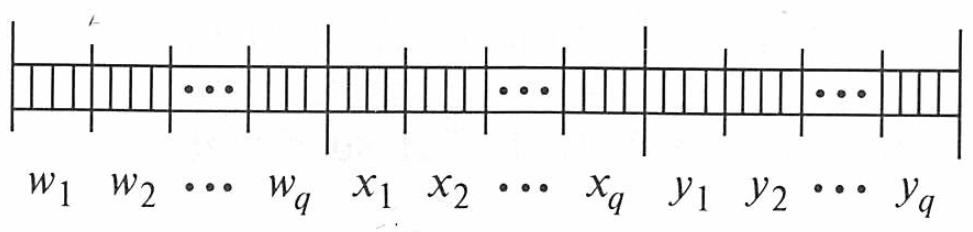
\includegraphics[width=.9\linewidth,height=.25\textheight,keepaspectratio]{Tabla}
    \caption{representación de las 3q zonas con p bits cada una}
    \label{fig:my_label}
\end{figure}

Una vez se han construido las $3q$ zonas de $p$ bits para una tripleta $m_i$, se marca con un 1 el bit menos significativo de cada una de las 3 zonas que corresponden a un elemento que está en dicha tripleta. Así, $s(a_i)$ se puede obtener expresando en base decimal el número binario resultante, o mediante la siguiente fórmula:

\[ s(a_i) = 2^{p(3q - f(i))} + 2^{p(2q - g(i))} + 2^{p(q - h(i)} \]

Siendo $f(i)$, $g(i)$ y $h(i)$ las funciones que devuelven los números entre 1 y $q$ que corresponden a las zonas asignadas a cada elemento de la tripleta $i$. Las funciones $f$, $g$ y $h$ están asociadas a los conjuntos $W$, $X$ e $Y$, respectivamente.

Cabe destacar que cada $s(a_i)$ se puede construir en tiempo polinomial a partir de la entrada de 3DM, dado que, para representar cada uno en binario, se usa un máximo de $3pq$ bits.

La construcción de la representación binaria de los $s(a)$ se ha realizado de forma que, si se suman los valores de todas las $k$ tripletas de las zonas que corresponden a un mismo elemento, el resultado nunca superará $k = 2^p - 1$, por lo que nunca se producirá un overflow al sumar. 

Así, se construye un número auxiliar $B$, cuya representación binaria contiene un 1 en la posición menos significativa de cada una de sus $3q$ zonas. Se puede calcular con la siguiente fórmula:

\[ B = \sum_{j = 0}^{3q - 1} 2^{pj}\]

El número $B$ también se puede obtener sumando los $s(a)$ de un conjunto $A' \subseteq A$ de tripletas, si y solo si estas constituyen un matching, es decir, una solución del problema 3DM de entrada. 

En segundo lugar, se debe de calcular los dos números restantes ($s(b_1), s(b_2)$) que vamos a añadir al conjunto $A$.
Para calcular ambos números, debemos de calcular el sumatorio de los números primeros $k$ números de A y el elemento $B$ como hemos mencionado ya.

El sumatorio de los primeros $k$ elementos se calcula de la siguiente manera.

\[\sum_{i=1}^{k}s(a_{i})\]

Y para calcular los dos últimos elementos de A se utilizan las siguiente fórmula:

\[ s(b_1) = 2 \left[\sum_{i=1}^{k}s(a_{i})\right] - B \quad s(b_2) = \left[\sum_{i=1}^{k}s(a_{i})\right] + B\]

Ambas sumas pueden ser representadas por $3qp + 1$ bits en tiempo polinomial, dada la entrada del problema 3DM.
Si la entrada 3DM contenía un matching tridimensional, entonces existe \(A' \subseteq A\), tal que \[ \sum_{a\in A'}s(a)= \sum_{a\in A - A'}s(a)\]

Si se cumple esta condición, las sumas de ambas será de \(2\sum_{i=1}^{k}s(a_{i})\), y uno de los conjuntos, $A'$ o $A-A'$, tendrá $b_1$ pero no $b_2$, que estará en el otro conjunto. Con esto en mente, si sabemos que $B$ es la suma de los $s(a)$ de las tripletas que son una solución del problema 3DM, y sabemos que la suma de ambos conjuntos será \(2\sum_{i=1}^{k}s(a_{i})\), podemos afirmar que el conjunto A', estará formado por \(\{b_1\} \cup \{a_i : m_i \in M'\}\).
\newline

Como estas transformaciones a números decimales, se pueden hacer en tiempo polinomial con no más de $(3qp + 1)$ bits cuyos parámetros vienen dados por el problema 3DM, podemos confirmar que  \(3DM \ \preceq \ PARTITION\) y se prueba la NP-Completitud del segundo. 
\end{proof}

\end{document}